
\newcommand{\DBIndex}{DBIndex}
\newcommand{\blockset}{{\cal B}}
\newcommand{\clusterset}{{\cal C}}

\section{Dense Block Index}
A straightforward approach to process a graph window query 
$Q = (G, W, \Sigma, A)$, where $G = (V,E)$,
is to dynamically compute the window $W(v)$ for each vertex $v \in V$ and
its aggregation 
$\Sigma_{v' \in W(v)} v'.A$ 
independently from other vertices. We refer to this approach as \emph{Non-Indexed} method.

Given that many of the windows would share many common nodes (e.g., the k-hop windows of two adjacent nodes),
such a simple approach would be very inefficient due to the lack of sharing of the aggregation computations. 

To efficiently evaluate graph window queries, we propose an indexing technique named \emph{dense block index} (\textit{\DBIndex}), which is both space and query efficient. 
The main idea of \DBIndex\ is to try to reduce the aggregation computation cost by identifying subsets of nodes that are shared by more than one window 
so that the aggregation for the shared nodes could be computed only once instead of multiple times.

For example, consider a graph window query on the social graph in Fig.~\ref{fig:attributed} using the 1-hop window function.
We have $W(B) = \{A,B,D,F\}$ and $W(C) = \{A,C,D,E,F\}$ sharing three common nodes $A$, $D$, and $F$.
By identifying the set of common nodes $S=\{A,D,F\}$, its aggregation 
$\Sigma_{v \in S} v.A$ can be computed only once
and then reuse to compute the aggregation for $\Sigma_{v \in W(B)} v.A$ and $\Sigma_{v \in W(C)} v.A$.

%Given a graph window query $Q = (G, W, \Sigma, A)$ on a graph $G=(V,E)$,
Given a window function $W$ and a graph $G=(V,E)$,
we refer to a non-empty subset $B \subseteq V$ as a {\it block}.
Moreover, if $B$ contains at least two nodes and $B$ is contained by at least two different windows
(i.e., there exists $v_1, v_2 \in V$, $v_1 \neq v_2$, $B \subseteq W(v_1)$, and $B \subseteq W(v_2)$),
then $B$ is referred to as a {\it dense block}.
Thus, in the last example, $\{A,D,F\}$ is a dense block.

We say that a window $W(X)$ is {\it covered} by a collection of disjoint blocks $\{B_1,\cdots,B_n\}$
if the set of nodes in the window $W(X)$ is equal to the union of all nodes in the collection of disjoint blocks;
i.e., $W(X) = \bigcup_{i=1}^{n} B_i$ and $B_i \cap B_j = \emptyset$ if $i \neq j$.

To maximize the sharing of aggregation computations for a graph window query, 
the objective of \DBIndex\ is to identify a small set of blocks $\blockset$ such that
for each $v \in V$, $W(v)$ is covered by a small subset of disjoint blocks in $\blockset$.
Clearly, the cardinality of $\blockset$ is minimized if $\blockset$ contains a few large dense blocks.

Thus, given a window function $W$ and a graph $G=(V,E)$,
%given a graph window query $Q = (G, W, \Sigma, A)$ on a graph $G=(V,E)$,
a \DBIndex\ to evaluate $W$ on $G$ consists of three components in the form of a bipartite graph.
The first component is a collection of nodes (i.e., $V$);
%The first component is a collection of windows; i.e., $\{W(v) |\ v \in V\}$;
the second component is a collection of blocks; i.e., $\blockset = \{B_1,\cdots,B_n\}$ where each $B_i \subseteq V$;
and the third component is a collection of links from blocks to nodes
such that if a set of blocks $B(v) \subseteq \blockset$ is linked to a node $v \in V$,
then $W(v)$ is covered by $B(v)$.
Note that a \DBIndex\ is independent of both the aggregation function (i.e., $\Sigma$) and the attribute to be aggregated (i.e., $A$).

Fig.~\ref{fig:dbi_agg}(a) shows an example of a \DBIndex\ wrt the social graph in Fig.~\ref{fig:attributed} and the 1-hop window function.
Note that the index consists of a total of seven blocks of which three of them are dense blocks.

\begin{figure}[t]
\centerline{
	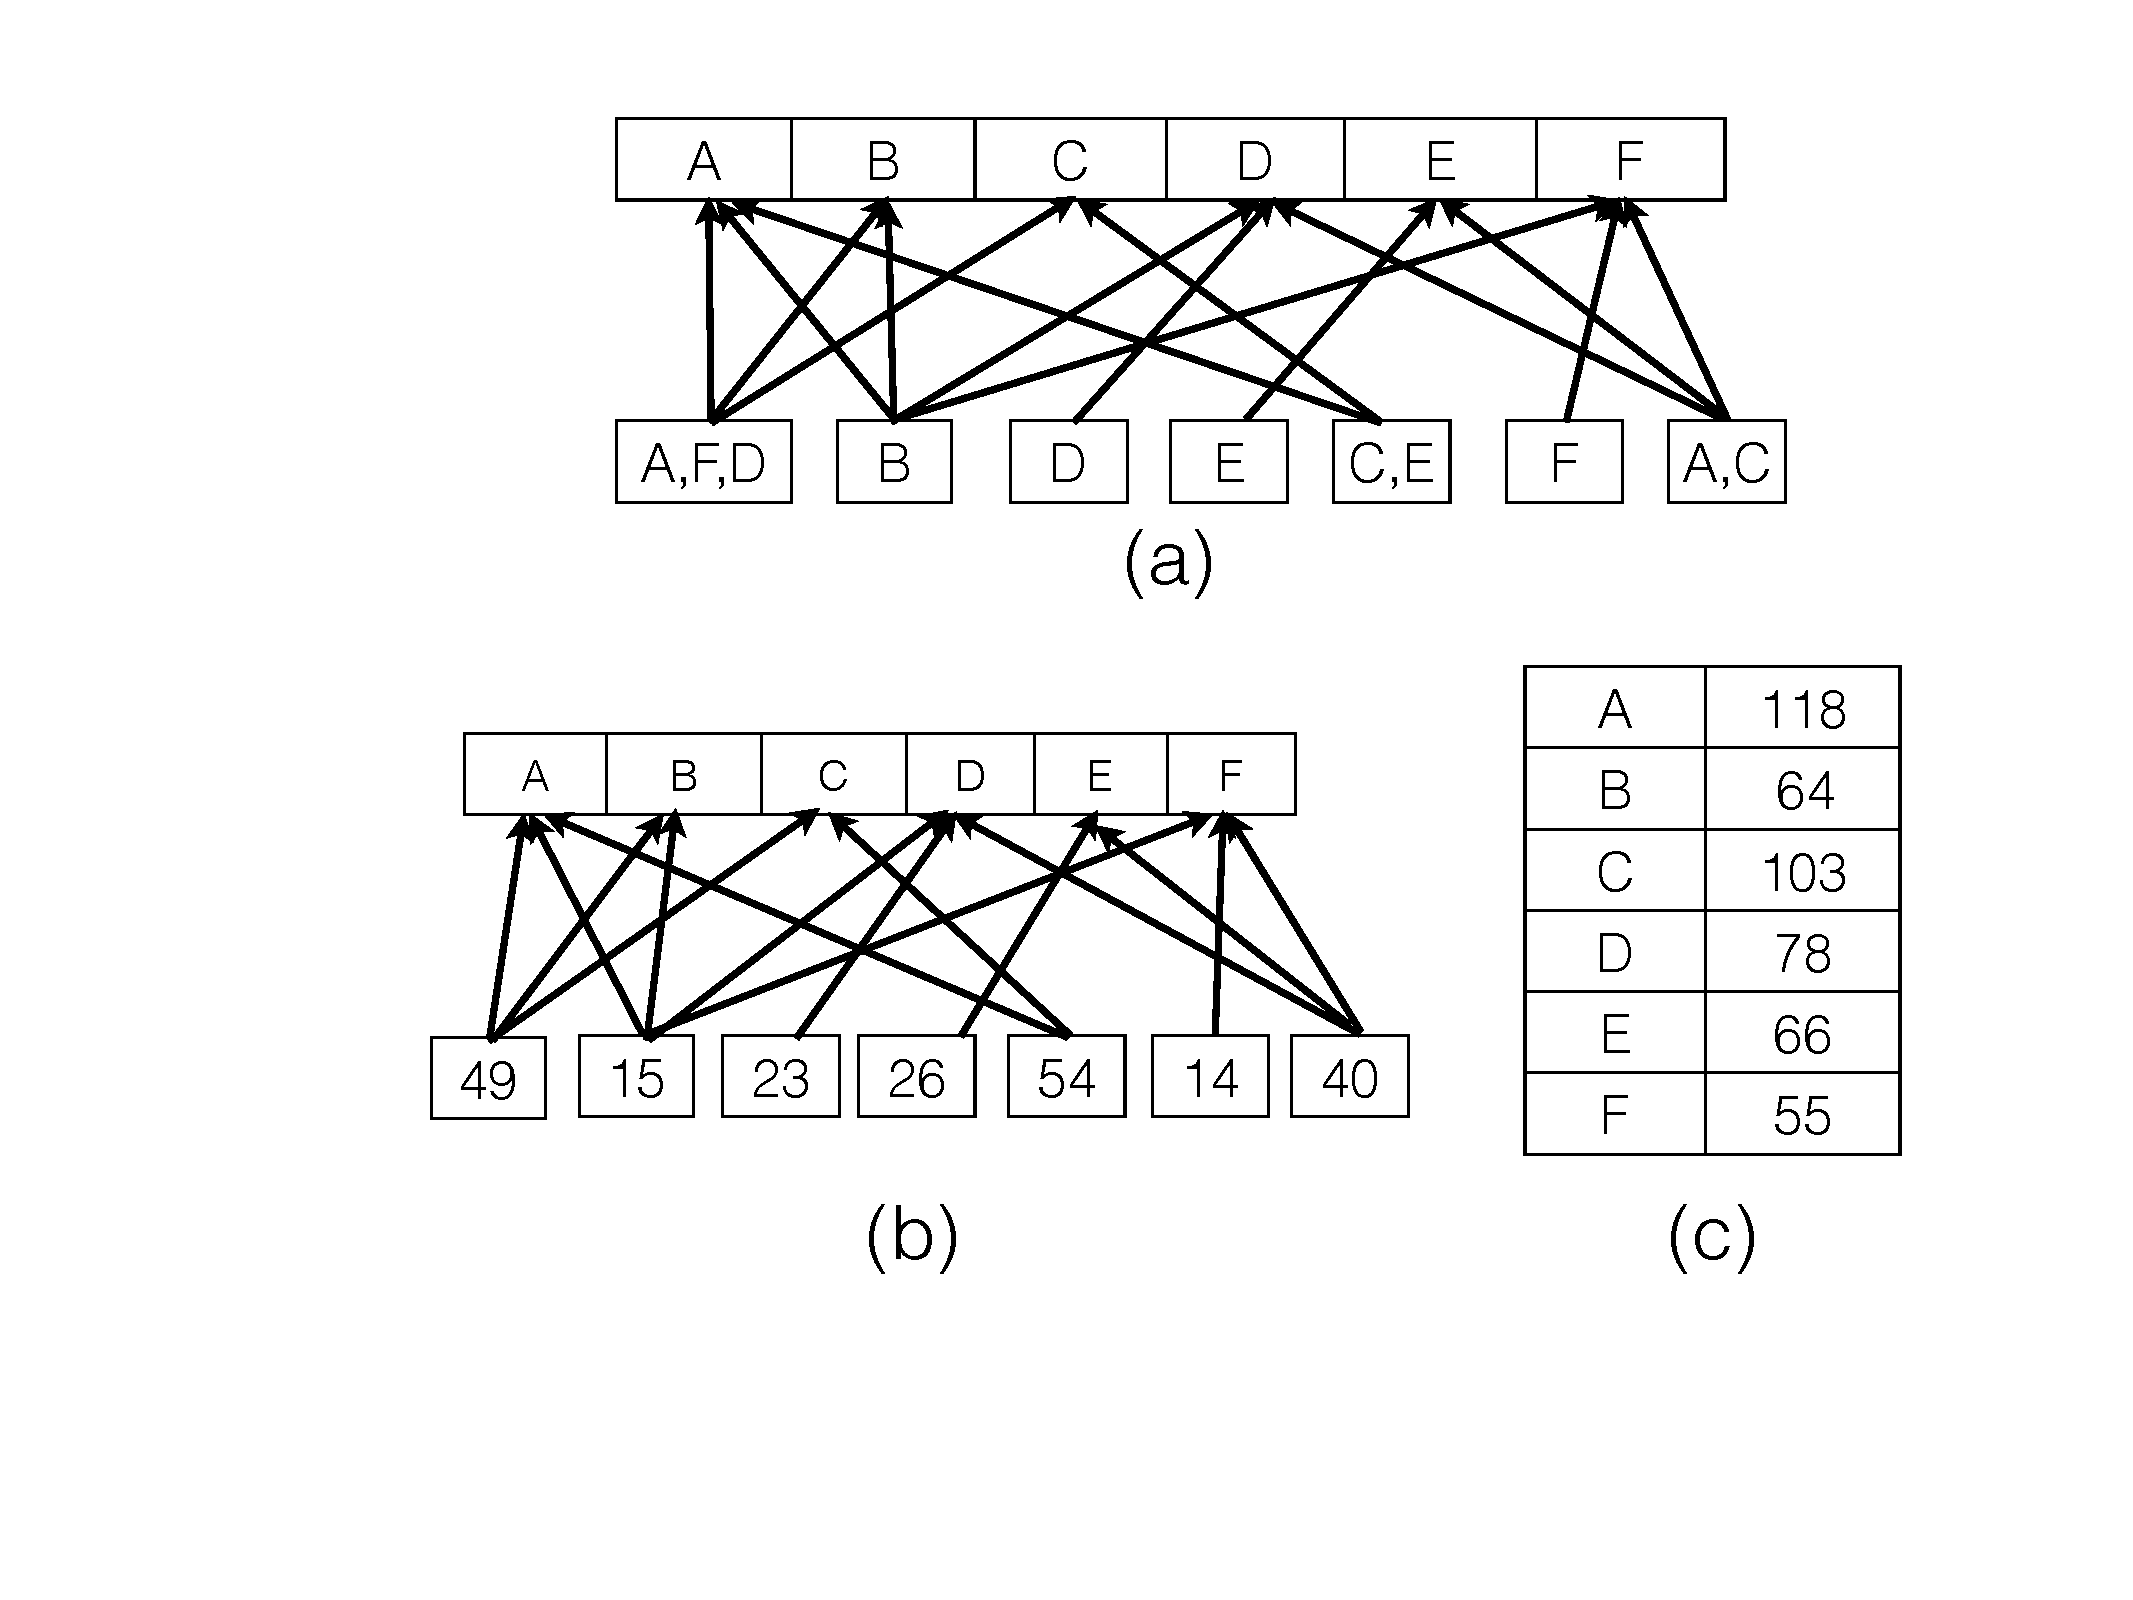
\includegraphics[width=0.8\textwidth]{chapter3/dbi_process} 
	}
	\caption{Window Query Processing using DBIndex. (a) provides the DBIndex for 1-hop window query in Fig.~\ref{fig:attributed}; (b) shows the partial aggregate results based on the dense block; (c) provides the final aggregate value of each window. }
	\label{fig:dbi_agg}
\end{figure}

\subsection{Query Processing using \DBIndex}
Given a \DBIndex\ wrt a graph $G$ and a window function $W$, a graph window query $Q = (G, W, \Sigma, A)$ is processed by the following two steps.
First, for each block $B_i$ in the index, we compute the aggregation (denoted by $T_i$) over all the nodes in $B_i$;
i.e., $T_i = \Sigma_{v \in B_i} v.A$. 
Thus, each $T_i$ is a partial aggregate value.
Next, for each window $W(v)$, $v \in V$, the aggregation for the window is computed by aggregating over all the partial aggregates
associated with the blocks linked to $W(v)$;
i.e., if $B(v)$ is the collection of blocks linked to $W(v)$, 
then the aggregation for $W(v)$ is given by $\Sigma_{B_i \in B(v)} T_i$. 

Consider again the \DBIndex\ shown in Fig.~\ref{fig:dbi_agg}(a) 
defined wrt the social graph in Fig.~\ref{fig:attributed} and the 1-hop window function.
Fig.~\ref{fig:dbi_agg}(b) shows how the index is used to evaluate the graph window query $(G, W, sum, Posts)$
where each block is labeled with its partial aggregate value;
and
Fig.~\ref{fig:dbi_agg}(c) shows the final query results.




%%%%%%%%%%%%%%%%%%%%%%%%%%%%%%%%%%%%%%%%%%%%%%%%%%%%%%%%%%%%%%%%%%%%%%%%%%%%%%%
%%%%%%%%%%%%%%%%%%%%%%%%%%%%%%%%%%%%%%%%%%%%%%%%%%%%%%%%%%%%%%%%%%%%%%%%%%%%%%%
%%%%%%%%%%%%%%%%%%%%%%%%%%%%%%%%%%%%%%%%%%%%%%%%%%%%%%%%%%%%%%%%%%%%%%%%%%%%%%%
%%%%%%%%%%%%%%%%%%%%%%%%%%%%%%%%%%%%%%%%%%%%%%%%%%%%%%%%%%%%%%%%%%%%%%%%%%%%%%%
%%%%%%%%%%%%%%%%%%%%%%%%%%%%%%%%%%%%%%%%%%%%%%%%%%%%%%%%%%%%%%%%%%%%%%%%%%%%%%%

%%%%%%%%%%%%%%%%%%%%%%%%%%%%%%%%%%%%%%%%%%%%%%%%%%%%%%%%%%%%%%%%%%%%
\subsection{\DBIndex\ Construction} 

In this section, we discuss the construction of the \DBIndex\ (wrt a graph $G=(V,E)$ and window function $W$) which has two key challenges.

The first challenge is the time complexity of the index construction. 
From our discussion of query processing using DBIndex, we note that the number of aggregation computations is determined by both the number of blocks as well as the number of links in the index; 
the former determines the number of partial aggregates to compute
while the latter determines the number of aggregations of the partial aggregate values.
Thus, to maximize the shared aggregation computations using DBIndex, both the number of blocks in the index as well as the number of blocks covering each window should be minimized. 
%As discussed, to maximize the shared aggregation computations using \DBIndex,
%both the number of blocks in the index as well as the number of blocks covering each window should be minimized.
However, finding the optimal \DBIndex\ to minimize this objective is NP-hard\footnote{
Note that a simpler variation of our optimization problem has been proven to be NP-hard \cite{vassilevska2004finding}.}.
Therefore, efficient heuristics are needed to construct the \DBIndex.

The second challenge is the space complexity of the index construction.
In order to identify large dense blocks to optimize for query efficiency,
a straightforward approach  is to first derive the window $W(v)$ for each node $v \in V$ and
then use this derived information to identify large dense blocks.
However, this direct approach incurs a high space complexity of $O(|V|^2)$.
Therefore, a more space-efficient approach is needed in order to scale to handle large graphs.

In this section, we present two heuristic approaches, namely {\it MC} and {\it EMC}, to construct \DBIndex.
The second approach EMC is designed to improve the efficiency of the first approach MC for constructing \DBIndex\
(wrt k-hop window function) by using some approxmation techique at the expense of possibly sacrificing 
the ``quality'' of the dense blocks (in terms of their sizes).

%%%%%%%%%%%%%%%%%%%%%%%%%%%%%%%%%%%%%%%%%%%%%%%%%%%%%%%%%%%%%%%%
\subsubsection{MinHash Clustering (MC)}

To reduce both the time and space complexities for the index construction,
instead of trying to identify large dense blocks among a large collection of windows,
we first partition all the windows 
into a number of smaller clusters of similar windows and then identify large dense blocks for each of the smaller clusters.
Intuitively, two windows are considered to be highly similar if they share a larger subset of nodes.
We apply the well-known {\it MinHash based Clustering (MC)} algorithm \cite{broder1997syntactic} to partition the windows into clusters of similar windows.
The MinHash clustering algorithm is based on using the
\emph{Jaccard Coefficient} to measure the similarity of two sets.  
Given the two window $W(v)$ and $W(u)$, $u,v \in V$,
their \emph{Jaccard Coefficient} is given by
\begin{equation} \label{eq:jacc_sim}
	J(u,v) = \frac{|W(u) \cap W(v)|}{|W(u) \cup W(v)|}
\end{equation}
The \emph{Jaccard Coefficient} ranges from 0 to 1, where  a larger value means that the windows are more similar.

\begin{figure}[htb]
\centering
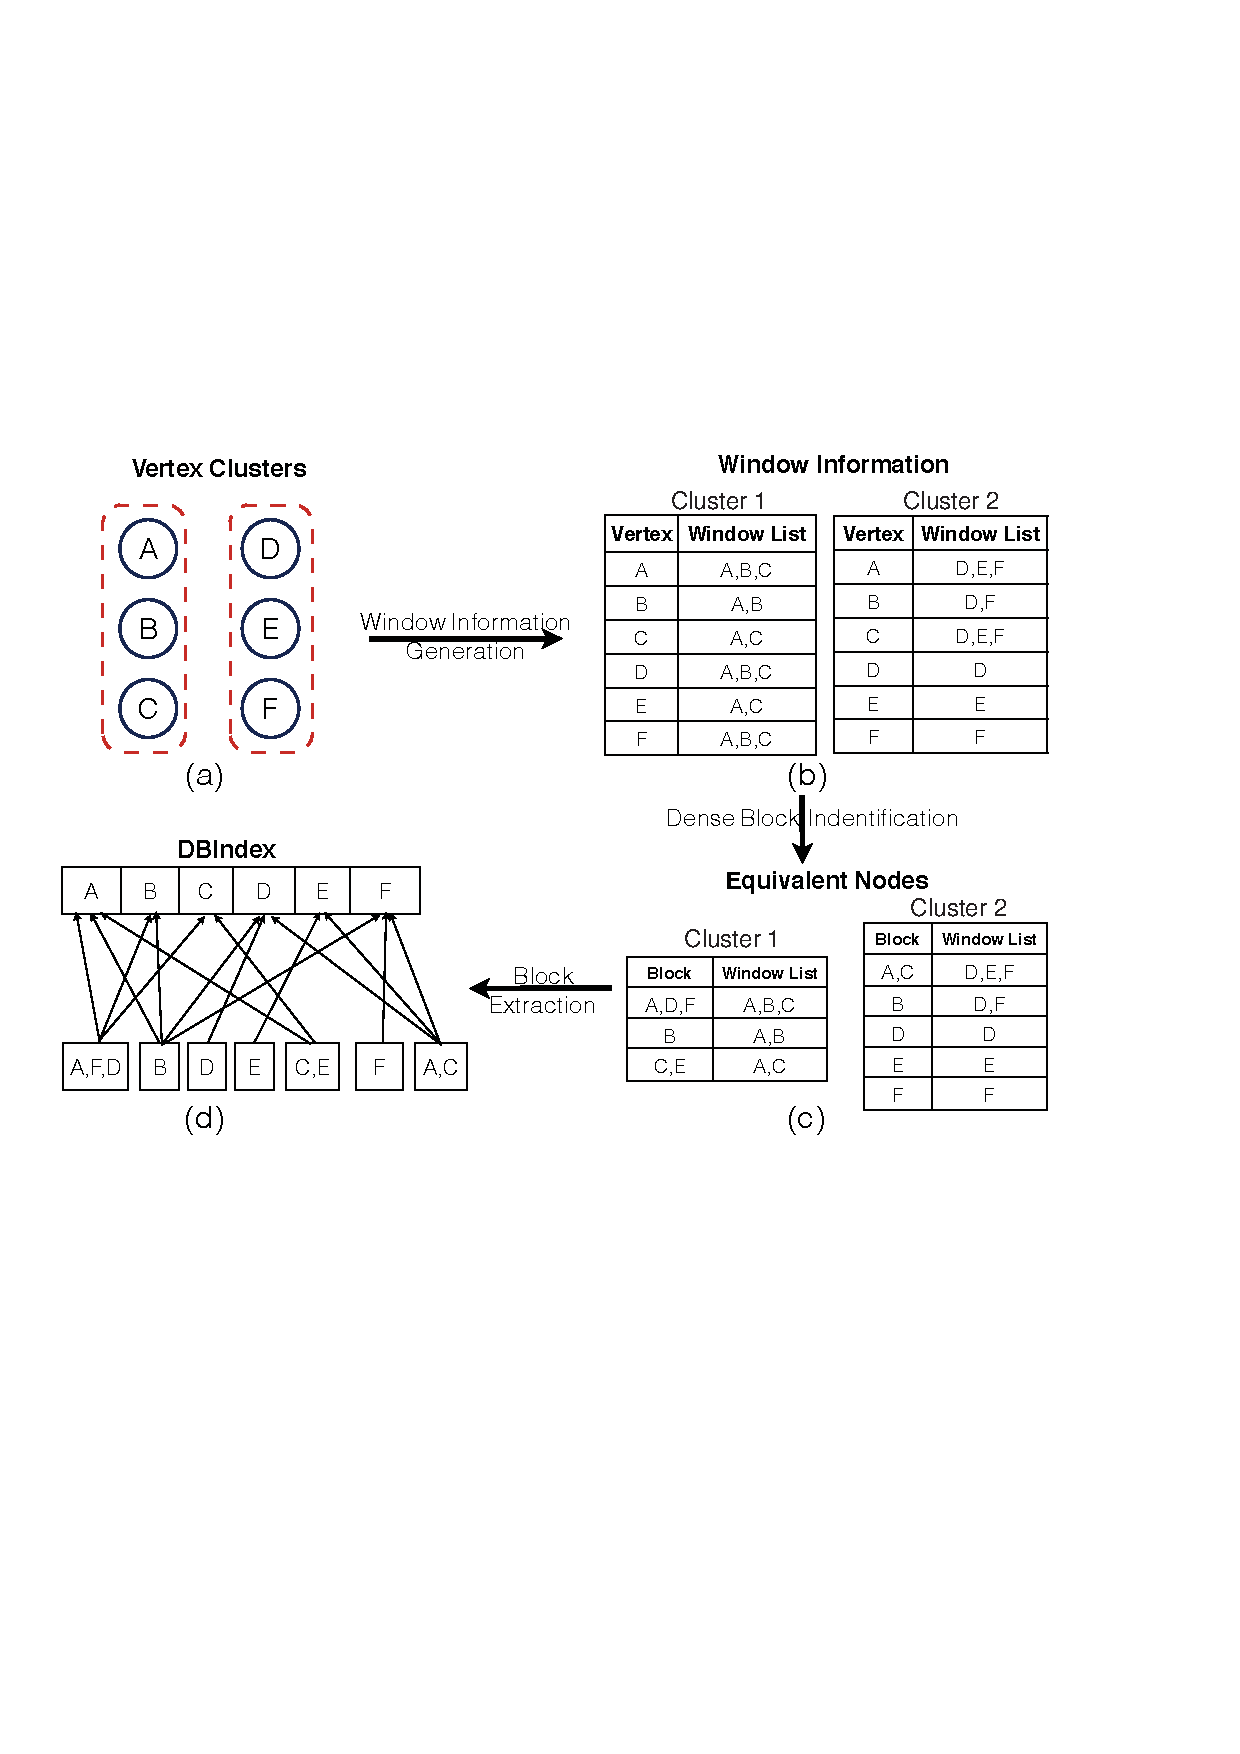
\includegraphics[width=0.8\textwidth]{chapter3/dbi_indexing.pdf}
\caption{DBIndex Construction over Social Graph in Fig.~\ref{fig:attributed}. (a) shows two clusters after MinHash clustering; (b) shows the window information of involved vertices within each cluster; (c) shows the dense blocks within each cluster; (d) provides the final DBIndex.}
\label{fig:dbi-indexing}
\end{figure}


Our heuristic approach to construct \DBIndex\ $I$ operates as follows.
Let $nodes(I)$, $blocks(I)$, and $links(I)$ denote, respectively,
the collection of nodes, blocks, and links that form $I$.
Initially, we have $nodes(I) = V$,
$blocks(I) = \emptyset$,
and
$links(I) = \emptyset$.
\begin{algorithm}
\caption{CreateDBIndex}
\begin{algorithmic}[1]  \small
%\FUNCTION $dbiGen$
\Require Graph $G=(V,E)$, window function $W$
\Ensure \DBIndex\ $I$
\State Initialize \DBIndex\ $I$: $nodes(I)=V$, $blocks(I)=\emptyset$, $links(I)=\emptyset$
\ForAll{$v \in V$}
	\State Traverse $G$ to determine $W(v)$
	\State Compute the hash signature $H(v)$ for $W(v)$
\EndFor
\State Partition $V$ into clusters $\clusterset = \{C_1,C_2,\cdots\}$ based on hash signatures $H(v)$
\ForAll{$C_i \in \clusterset$}
	\ForAll{$v \in C_i$} 
		\State Traverse $G$ to determine $W(v)$
	\EndFor
	\State {\tt IdentifyDenseBlocks} $(I,G,W,C_i)$
\EndFor
\Return $I$
\end{algorithmic}
\label{algo:k-hop-dbi}
\end{algorithm}

The first step is to partition the nodes in $V$ into clusters
using MinHash algorithm such that nodes with similar windows belong to the same cluster. 
For each node $v \in V$, we first derive its window $W(v)$ by an appropriate traversal of the graph $G$.
Next, we compute a hash signature (denoted by $H(v)$) for $W(v)$ based on applying $m$ hash functions on the set $W(v)$.
Nodes with identical hash signatures are considered to have highly similar windows and are grouped into the same cluster.
To ensure that our approach is scalable,
we do not retain $W(v)$ in memory  after its hash signature $H(v)$ has been computed and used to cluster $v$;
i.e., our approach does not materialize all the windows in the memory to avoid high space complexity.
Let $\clusterset = \{C_1,C_2,\cdots\}$ denote the collection of clusters obtained from the first step,
where each $C_i$ is a subset of nodes.
%A cluster is classified as {\it trivial} if it contains only one window; otherwise, it is classified as {\it non-trivial}.

The second step is to identify dense blocks from each of the clusters computed in the first step.
%For each cluster $C_i \in \clusterset$,
%let $N_i$ denote the union of all the nodes in all the windows in $C_i$;
%i.e., $N_i = \{v \in W(u) |\ W(u) \in C_i\}$.
The identification of dense blocks in each cluster $C_i$ is based on the notion of node equivalence defined as follows.
Two distinct nodes $u, v \in C_i$ are defined to be equivalent (denoted by $u \equiv v$)
if $u$ and $v$ are both contained in the same set of windows;
i.e., for every window $W(x), x \in C_i$, $u \in W(x)$ iff $v \in W(x)$.
Based on this notion of node equivalence, $C_i$ is partitioned into blocks of equivalent nodes.
To perform this partitioning, we need to again traverse the graph for each node $v \in C_i$ to 
determine its window $W(v)$\footnote{
Note that although we could have avoided deriving $W(v)$ a second time if we had materialzed all the derived windows the first time, our approach is designed to avoid the space complexity of materializing all the windows in memory at the cost of computing each $W(v)$ twice. We present an optimization in Section~\ref{sec:optimized} to avoid the recomputation cost.
}.
%However, since $C_i$ is now  a smaller cluster of nodes, we can now materialize all the windows for the nodes in $C_i$ in memory without exceeding the memory space.

However, since $C_i$ is now a smaller cluster of nodes, we can now materialize all the windows for the nodes in $C_i$ in memory without exceeding the memory space. In the event that a cluster $C_i$ is still too large for all its vertex windows to be materialized in main memory, we can further partition $C_i$ into equal size sub-clusters. This re-partition process can be recursively performed until the sub clusters created are small enough such that the windows for all nodes in the sub clusters fit in memory. 


Recall that a block $B$ is a dense block if $B$ contains at least two nodes and
$B$ is contained in at least two windows.
Thus, we can classify the nodes in each $C_i$ as either dense or non-dense nodes:
a node $v \in C_i$ is classified as a {\it dense node} if $v$ is contained in a dense block;
otherwise, $v$ is a non-dense node.

For each dense block $B$ in $C_i$,
we update the blocks and links in the \DBIndex\ $I$ as follows:
we insert $B$ into $blocks(I)$ if $B \not\in blocks(I)$,
and we insert $(B,v)$ into $links(I)$
for each $v \in C_i$ where $B \subseteq W(v)$.
If all the blocks in $C_i$ are dense blocks, then we are done with identifying dense blocks in $C_i$;
otherwise, there are two cases to consider.
%otherwise, we update $C_i$ by removing all the dense nodes from $C_i$ and recursively apply the
%two-step procedure on the updated $C_i$ to try to identify more dense blocks.
For the first case, if all the nodes in $C_i$ are non-dense nodes,
then we also terminate the process  of identifying dense blocks in $C_i$
and update the blocks and links in the \DBIndex\ $I$ as before:
we insert each non-dense block $B$ into $blocks(I)$,
and we insert $(B,v)$ into $links(I)$ for each $v \in C_i$ where $B \subseteq W(v)$.
For the second case, if $C_i$ has a mixture of dense and non-dense nodes,
we remove the dense nodes from $C_i$ and recursively identify dense blocks in $C_i$
following the above two-step procedure.

Note that since the blocks are identified independently from each cluster,
it might be possible for the same block to be identified from different clusters.
We avoid duplicating the same block in $blocks(I)$ by checking that a block $B$ is not already in $blocks(I)$
before inserting it into $blocks(I)$.
The details of the construction algorithm are shown as Algorithms
\ref{algo:k-hop-dbi},
\ref{algo:identify},
and
\ref{algo:refine}.

%begin{algorithm}
%\caption{IdentifyDenseBlocks}
%\begin{algorithmic}[1]
%\REQUIRE \DBIndex\ $I$, Graph $G=(V,E)$, window function $W$, a cluster $C_i \subseteq V$
%%\ENSURE \DBIndex
%\STATE Partition $C_i$ into blocks based on node equivalence
%\STATE Initialize $DenseNodes = \emptyset$
%\FORALL{dense block $B$}
% \STATE Insert $B$ into $blocks(I)$ if $B \not\in blocks(I)$
% \STATE Insert $(B,v)$ into $links(I)$ for each $v \in C_i$ where $B \subseteq W(v)$
% \STATE $DenseNodes = DenseNodes \cup B$
%\ENDFOR
%\IF{($DenseNodes = \emptyset$)}
% \FORALL{block $B$}
%  \STATE Insert $B$ into $blocks(I)$ if $B \not\in blocks(I)$
%  \STATE Insert $(B,v)$ into $links(I)$ for each $v \in C_i$ where $B \subseteq W(v)$
% \ENDFOR
%\ELSIF{($C_i - DenseNodes \neq \emptyset$)}
% \IF{($C_i \neq DenseNodes$)}
%  \STATE {\tt RefineCluster} $(I,G,W,C_i - DenseNodes)$
%  \ENDIF
%\ENDIF
%\end{algorithmic}
%\label{algo:identify}
%\end{algorithm}

\begin{algorithm}
\caption{IdentifyDenseBlocks}
\begin{algorithmic}[1] \small
\Require \DBIndex\ $I$, Graph $G=(V,E)$, window function $W$, a cluster $C_i \subseteq V$
%\ENSURE \DBIndex
\State Partition $C_i$ into blocks based on node equivalence
\State Initialize $DenseNodes = \emptyset$
\ForAll{dense block $B$}
	\State Insert $B$ into $blocks(I)$ if $B \not\in blocks(I)$
	\State Insert $(B,v)$ into $links(I)$ for each $v \in C_i$ where $B \subseteq W(v)$
	\State $DenseNodes = DenseNodes \cup B$
\EndFor
\If{($DenseNodes = \emptyset$)}
	\ForAll{block $B$}
		\State Insert $B$ into $blocks(I)$ if $B \not\in blocks(I)$
		\State Insert $(B,v)$ into $links(I)$ for each $v \in C_i$ where $B \subseteq W(v)$
	\EndFor
\ElsIf{($C_i - DenseNodes \neq \emptyset$)}
	\If{($C_i \neq DenseNodes$)}
		\State {\tt RefineCluster} $(I,G,W,C_i - DenseNodes)$
	\EndIf
\EndIf
\end{algorithmic}
\label{algo:identify}
\end{algorithm}

Fig.~\ref{fig:dbi-indexing} 
illustrates the construction of the DBIndex with respect to the social graph in 
Fig.~\ref{fig:attributed}(a) and 1-hop window using the MC algorithm.
First, the set of graph vertices are partitioned into clusters using MinHash clustering;
Fig.~\ref{fig:dbi-indexing}(a)
shows that the set of vertices $V = \{A, B, C, D, E, F \}$ are partitioned into two clusters $C_1=\{A, B, C\}$ and $C_2=\{D, E, F\}$. 

For convenience, cluster 1 in 
Fig.~\ref{fig:dbi-indexing}(b) shows for each $v \in C_1$, the set of vertices whose windows contain $v$;
i.e., $\{u |\ v \in W(u)\}$.
Similarly, Cluster 2 in Fig.~\ref{fig:dbi-indexing} (b)
shows for each $v \in C_2$, the set of vertices whose windows contain $v$.
Consider the identification of dense blocks in cluster $C_1$.
As shown in Fig.~\ref{fig:dbi-indexing} (c), based on the notion of equivalence nodes,
cluster $C_1$ is partitioned into three blocks of equivalent nodes:
$B_1=\{A,D,F\}$, $B_2=\{B\}$, and $B_3\{C,E\}$.
Among these three blocks, only
$B_1$ and $B_3$ are dense blocks.
The MC algorithm then tries to repartition the window $A,B,C$ using non-dense nodes in $C_1$,
(i.e., $B_2$). Since $B_2$ is the only non-dense node, it directly outputs.
%the remaining non-dense nodes in $C_1$ (i.e., $\{B\}$).
At the end of processing cluster $C_1$,
the DBIndex $I$ is updated as follows:
$blocks(I) = \{B_1, B_2, B_3\}$ 
and
$links(I) = \{ (B_1,\{A,B,C\}), (B_2, \{A,B\}),$, $(B_3, \{A,C\}) \}$. The identification of dense blocks in cluster $C_2$ 
is of similar process.

We find it is non-trivial to precisely analyze the complexity of Algorithm~\ref{algo:k-hop-dbi}. Here, we only offer a brief analysis. Suppose the MinHash cost is $H$ and the total cost for k-bounded BFS for all vertex is $B$, Lines 1-5 has the complexity of $O(H + B)$.  Lines 7-10 has the complexity of $O(B)$. A single execution of Algorithm~\ref{algo:identify}  has the  complexity of $O(|V|)$, since we can simply partition nodes using hashing. Suppose the iteration runs for $K$ times, the total cost for Algorithm~\ref{algo:identify} and Algorithm~\ref{algo:refine} is $O(K|V|)$. Therefore the overall complexity of Algorithm~\ref{algo:k-hop-dbi} is $O(H+2*B + O(K|V|))$. $H$ depends on the number of vertex-window mappings for a given query and $B$ depends on the graph structure and number of hops. As we demonstrate in Section 6, the $H$ and $B$ are the major contribution of the indexing time. To reduce the index time, we provide further optimization techniques.


\begin{algorithm}
\caption{RefineCluster}
\begin{algorithmic}[1]
\Require \DBIndex\ $I$, Graph $G=(V,E)$, window function $W$, a cluster $C \subseteq V$
%\ENSURE \DBIndex
\ForAll{$v \in C$}
	\State Compute the hash signature $H(v)$ for $W(v) \cap C$
\EndFor
\State Partition $C$ into clusters $\clusterset = \{C_1,C_2,\cdots\}$ based on hash signatures $H(v)$
\ForAll{$C_i \in \clusterset$}
	\State {\tt IdentifyDenseBlocks} $(I,G,W,C_i)$
\EndFor
\end{algorithmic}
\label{algo:refine}
\end{algorithm}
%%%%%%%%%%%%%%%%%%%%%%%%%%%%%%%
\eat{
We adopt the \emph{MinHash} clustering  
\cite{broder1997syntactic} 
in index construction to discover the dense blocks. MinHash has been well known for its effectiveness of set clustering by using the Jaccard Coefficient. Our proposed MC approach to generate the index as follows: First, k min-wise independent functions are used to generate $k$ hash signatures for each window. Note that this is a general procedure in MinHash clustering. As all the vertex window mapping is large, we avoid materializing this mapping by dynamically computing the window for each vertex. The k-hop window collection for one vertex can be easily done by using the KBBFS. Once each window is collected, its $k$ hash signatures will be generated. We emphasize that once the signatures are generated, the window information can be safely erased from to memory. To store the signatures, it can be stored in a signature matrix in $V \times k$, where cell $(i,j)$ records the $j^{th}$ hash signature of window $i$. The signature matrix is then sorted based on the row values. 



The first step clustering is conducted based on the sorted signature matrix. All the similar rows are clustered together. This clustering helps us identify all the similar windows. 

Within each cluster, we further perform a fine-grained similarity check to discover the dense blocks among the similar windows. To do this, for each cluster, we build one clustered matrix, where each column corresponds to one window in the cluster. The window information can be obtained by via the KBBFS using the vertex. Over each clustered matrix, we adopt an iterative indexing scheme. The scheme works as follows: for each cluster, we create a \emph{clustered matrix} whose column maps each member of cluster, and each column contains the value of that window. Given the clustered matrix, we sort the matrix based on rows, then merge the rows with identical value. The merged row indexes are effectively a dense block, thus can be output. For unmerged portion of the matrix, we use the similar \emph{MinHash} to cluster them, and pass the newly created clusters to the next iteration. In implementation, we can ignore all the zero rows, which is more space friendly. The index creation algorithm is shown as in Algo. \ref{algo:k-hop-dbi}. 



\begin{algorithm}
\caption{DBIGen - Iterative DBI Index Creation }
\begin{algorithmic}[1]
%\FUNCTION $dbiGen$
\REQUIRE $C$, \textbf{optional} $M$ \COMMENT{Window cluster, Lookup table}
\GLOBAL $DBI$ \COMMENT{Dense Block Index}
\STATE $DBI.window.add(C)$  \label{code:dbi-add-window}
\STATE $CW$ \COMMENT{Clustered window}
%\FORALL{$cluster \in C.clusters$} 
	\STATE $CW \leftarrow [\ ][\ ]$ \label{code:dbi-window-partition-start}
	\FORALL{$w \in C$}
		\STATE $CW[\ ][w] \leftarrow M[w]\ ||\ getWindow(w)$
	\ENDFOR \label{code:dbi-window-partition-end}
	\STATE sort $CW$ by $rows$ \label{code:dbi-sort}
	\FORALL{$row$ occurs twice in $rows$}
		\STATE $block.addAll(row.index)$ \label{code:dbi-add-block-start} \COMMENT{Create new block}
		\STATE $DBI.blocks.add(block)$
		\FOR{$col$ with value $CM[row][col]$ is 1}
			\STATE $DBI.links.add(col, block)$		
		\ENDFOR \label{code:dbi-add-block-end}
		\STATE $CW.remove(row)$ \label{code:dbi-remove-rows}
	\ENDFOR
	\FORALL{$c \in minHash(CW)$} \label{code:dbi-remain-min}
		\IF{$c.size > 2$}
			\STATE $dbiGen(c, CW)$ \label{code:dbi-recursive}
		\ENDIF
	\ENDFOR
%\ENDFOR
%\RETURN $DBI$
\end{algorithmic}
\label{algo:k-hop-dbi}
\end{algorithm}

Algo.~\ref{algo:k-hop-dbi} requires a cluster of window IDs as input. It optionally takes a lookup table from which the contents of a given window can be fetched. The algorithm starts with inserting window IDs into the window field of the global structure \emph{DBI}(Line~\ref{code:dbi-add-window}). Then $CW$ stores the clustered matrix for this cluster. It first attempts to get the information from the lookup table $M$, if failed, it calls $getWindow$ function which dynamically computes the window information. Then the $CW$ is sorted based on rows. For each rows with identical value, a dense block is created and recorded in \emph{DBI} (Line~\ref{code:dbi-add-block-start}-\ref{code:dbi-add-block-end}). Those rows then removed from $CW$ (Line~\ref{code:dbi-remove-rows}). The the remaining $CW$ is supplied to $minHash$ for clustering. For the new clusters with size greater than 2, it recursively calls Algo.~\ref{algo:k-hop-dbi}.
%%%%%%%%%%%%%%%%%%%%%%%%%%%%%%%%%%%%%%%%%%%%
%%%%%%%%%%%%%%%%%%%%%%%%%%%%%%%%%%%%%%%%%%%%
%%%%%%%%%%%%%%%%%%%%%%%%%%%%%%%%%%%%%%%%%%%%

In order to reduce the memory usage of Algo.~\ref{algo:k-hop-dbi}, a corner case needs to be taken care of. In Algo.~\ref{algo:k-hop-dbi}, a clustered matrix $CM$ is used temporarily to expand the window information for the cluster. If the clusters generated from the first minhash is too large, we need to split the cluster into equal size. The split works since it preserves the similarity measure, that is if a cluster contains similar elements, after split, each of the resulting cluster also contains similar elements. The split reduces the memory burden. In Line.~\ref{code:dbi-recursive}, the $CW$ is optionally passed to the minHash. Since $CW$ is already in memory, it can be passed to the next recursive call safely without causing memory issue.
 
The hashing results in a $V \times k$ matrix, with cell $(i,j)$ being the $j^{th}$ hash signature of window $i$. The matrix is then sorted in row major order and subsequently is traversed in column order. During traversal, rows with identical values are grouped into the same cluster. The hashing complexity is $O(k|nnz|+w|V|)$, where $w$ is cost for computing each window , the sorting is of complexity $O(k|V|log|V|)$, and the clustering is of complexity $O(|V|)$. Since $k$ is a small constant, the complexity of clustering algorithm is of $O(w|V|+|nnz|+|V|log(|V|))$. 

An example of \emph{MinHash} based \emph{DBIndex Indexing} is shown in Fig.~\ref{fig:dbi-indexing}. The top left part is the \emph{1-hop} window matrix for a attributed graph. The top right part is the partition result based on \emph{MinHash}. The bottom right part is the dense blocks identified by row condensing. And the bottom left part is the \emph{DBI} created based on the dense blocks.
}



%%%%%%%%%%%%%%%%%%%%%%%%%%%%%%%%%%%%%
%%%%%%%%%%%%%%%%%%%%%%%%%%%%%%%%%%%%%
%%%%%%%%%%%%%%%%%%%%%%%%%%%%%%%%%%%%%
%%%%%%%%%%%%%%%%%%%%%%%%%%%%%%%%%%%%%

\subsubsection{Estimated MinHash Clustering (EMC)}
\label{sec:optimized}
%\subsection{DBIndex Construction based on Estimated MinHash Clustering}

The MC approach described in the previous section requires the window of each node (i.e., $W(v), v \in V$)
to be computed twice in order to avoid the high space complexity of materializing all the windows in main memory.
For k-hop window function with a large value of $k$, the cost of graph traverals to compute the k-hop windows
could incur a high computation overhead. Moreover, the cost of initial MinHash in MC approach equals to the initial number of vertex-window mappings, which is of the same order as graph traversal. For the larger hops, MinHash clustering would incur high computation cost.

To address these issues, we present an even more efficient approach,
referred to as {\it Estimated MinHash Clustering (EMC)}, 
to optimize the construction of the \DBIndex\ for k-hop window function with larger k.

The key idea behind $EMC$ is based on the observation that for any two nodes $u, v \in V$,
if their $m$-hop windows, $W_m(u)$ and $W_m(v)$, are highly similar 
and they are grouped into the same cluster, 
then it is likely that the $n$-hop windows of these two nodes, where $n > m$,
would also be highly similar and grouped into the same cluster.

Using the above observation, we could reduce the overhead cost for constructing a \DBIndex\ wrt a $k$-hop window 
function by clustering the nodes based on their $k'$-hop windows, where $k' < k$, instead of their $k$-hop windows.

To reduce the overhead of window computations,
our $EMC$ approach is similar to the MC approach except   
for the first round of window computations
(line 3 in Algorithm \ref{algo:k-hop-dbi}):
$EMC$ uses lower hop windows to approximate $k$-hop windows for the purpose of clustering the nodes in $V$.
Thus, the hash signatures used for partitioning $V$ are based on lower hop windows.
This approximation clearly has the advantage of improved time-efficiency as traversing and Minhashing on lower hop window is of
order of magnitude faster. For the extreme case, adapting 1-hop window of a node $v$ requires only accessing the adjacent nodes of $v$. 
The tradeoff for this improved efficiency is that the ``quality'' of the dense blocks might be reduced (in terms of their sizes).
However, our experimental results show that this reduction in quality is actually only marginal which makes this approximation a worthy tradeoff.


\subsubsection {Justification of Heuristic}
In the following, we show the theoretical justification of our heuristic: the Jaccard coefficient
is increasing wrt number of hops for a large class of graphs. We 
assume that the degree of vertices follows the same distribution, which is true in most
real-networks and random graph models\footnote{E.g. Social network, Preferential Attachment model etc. follow
power-law distribution. However, our analysis do not restrict on power-law distribution.}.  
This implies we can analyze vertices 
with their neighborhoods structure using a unified way. 

We use $d_i$ to indicate the degree of vertex $i$. For any vertex pair $(u,v)$, their 
intersection on $k$-hop window consists of three part. We name them using $A=W_k(u)-W_k(v)$, 
$B=W_k(v)-W_k(u)$ and $C_k = W_k(u) \cap W_k(v)$. Clearly the Jaccard coefficient at $k$-hops
can be expressed as follows:
\begin{equation}
	J_k(u,v) = \frac{|C_k|}{|A_k| + |B_k| + |C_k|}
\end{equation}

To deduct the relationship between $J_k(u,v)$ and $J_{k+1}(u,v)$, we prove the following lemma first:
\begin{theorem}
Let $S$ be a collection of connected vertices, the number of newly discovered
vertices by one-hop expansion from $S$ is bounded by a function on $|S|$.
\end{theorem}
\begin{proof}
Consider a random variable $Y_i$ indicate the newly 
discovered vertices from one-hop expansion from vertex $i$. 
Then the probability of $|Y_i|=y$ is can be analyzed as follows: there 
are $d_i$ edges for vertex $i$. Since $|Y_i|$ is connected with $S$, one edge
is fixed to link with a vertex in $S$. There are remaining $d_i-1$ edges with
$y$ edges linked to the new vertices. In total, there are $|V|-1 \choose d_i -1$
combinations with $d_i$ edges. Therefore, the probability can be written as:
\begin{equation}
Prob(Y_i = y| v_i \in S) = \frac{{|S| -1 \choose d_i - y -1}{|V|-|S| \choose y}}{{|V|-1 \choose d_i -1}}
\end{equation}
Thus, the expectation of $Y_i$ is:
\begin{equation}
\begin{split}
E(Y_i|v_i \in S) & = \Sigma( y * Prob(Y_i = y| v_i \in S) )\\
	& = \Sigma_{y=1}^{y=d_i -1} ( \frac{{|S| -1 \choose d_i - y -1}{|V|-|S| \choose y}}{{|V|-1 \choose d_i -1}} * y )\\
	& = \Sigma_{y=1}^{y=d_i -1} (\frac{{|S| -1 \choose d_i - y -1}{|V|-|S| -1 \choose y - 1}}{{|V|-1 \choose d_i -1}} * (|V|-|S|))\\
	& = (|V|-|S|) * \Sigma_{y=1}^{y=d_i -1}\frac{{|S| -1 \choose d_i - y -1}{|V|-|S| -1 \choose y - 1}}{{|V|-1 \choose d_i -1}} \\
	& = (|V|-|S|) * \frac{{|V|-2 \choose d_i - 2}}{{|V|-1 \choose d_i -1}} = \frac{(|V|-|S|)*(d_i-1)}{|V| - 1}
\end{split}
\end{equation}
Taking the expectation over all vertices in $S$, we can find the expectation of $E(Y|S) = \frac{(|V|-|S|)*(\overline{d}-1)}{|V| - 1}$, 
where $\overline{d}$ is the average degree of the graph. We then define the event $X=\cup_{i=1}^{i=|S|} Y_i$, i.e. $X$ is the number
of newly discovered vertices for one-hop expansion of entire $S$. By union bound, 
the expectation of $X$ is:
\begin{equation} 
\begin{split}
E(X|S) &= E(\cup_{i=1}^{i=|S|}Y_i|S) \\
& \leq \Sigma_{i=1}^{i=|S|}E(Y_i|S) \\ 
&= \frac{|S|(|V|-|S|)(\overline{d} -1)}{|V|-1} = f(|S|)
\end{split}
\end{equation}
The bound is achieved when each vertices in $S$ discovers non-overlapping neighbors, such
as in the case of tree structure. Therefore, the newly discovered vertices are tightly bounded 
by a quadratic function on $|S|$.
\qed
\end{proof}

We thus use $f(m)$ to denote the number of newly discovered vertices
from a base set of $m$ connected vertices. Since $u,v$ have 
identical degree distribution, their expected value $S_u=E(|W_k(u)|)$
and $S_v=E(|W_k(v)|)$ is likely to be the same, i.e. $S_u \cong S_v$.
We further use $\alpha = \frac{|C|}{|A|+|C|}$ to denote the portion of shared
components in $u$'s $k$-hop neighborhood. Likewise, we use $\beta = \frac{|B|}{|B|+|C|}$ for 
$W_k(v)$. Since vertices have identical degree distribution, $\alpha$ and $\beta$ are likely
to be the same, i.e. $\alpha \cong \beta$.
Now, the $J_{k+1}(u,v)$ for ($k+1$)-hop can be represented as follows:
\begin{equation}
\begin{split}
J_{k+1}(u,v) & = \frac{|C_{k+1}|}{|A_{k+1}| + |B_{k+1}| + |C_{k+1}|} \\
	& = \frac{|C_k| + \alpha * f(S_u) + \beta * f(S_v)}{|A_k| +|B_k| +|C_k| +f(S_u) +  f(S_v) -\Delta} 
\end{split}
\end{equation}
, the $\Delta$ here is to compensate the doubly counted portion on the
overlapping: $(A_{k+1} \cup B_{k+1}) \cap C_{k+1}$. Therefore, it subsequently follows:
\begin{equation}
\begin{split}
J_{k+1}(u,v) & \geq \frac{|C_k| + \alpha * f(S_u) + \beta * f(S_v)}{|A_k| +|B_k| +|C_k| +f(S_u) +  f(S_v)}  \\
		& \cong \frac{|C_k| + 2\alpha * f(S_u)}{|A_k|+|B_k|+|C_k| + 2 * f(S_u)}
\end{split}
\end{equation}
Due to the fact that $\alpha = \frac{|C_k|}{|C_k|+|A_k|} \geq \frac{|C_k|}{|A_k|+|B_k|+|C_k|}$, it follows:
\begin{equation}
\begin{split}
	\frac{\alpha f(S_u)}{f(S_u)} & \geq \frac{|C_k|}{|A_k|+|B_k|+|C_k|} \Leftrightarrow \\
	\frac{|C_k| + 2\alpha * f(S_u)}{|A_k|+|B_k|+|C_k| + 2 * f(S_u)} & \geq \frac{|C_k|}{|A_k|+|B_k|+|C_k|} \\
	& = J_k(u,v)
\end{split}
\end{equation}

Therefore, our analysis shows that $J_k(u,v)$ is most likely increasing for random graphs with identical
degree distribution.

%If each $d_i$ follows the same distribution, we have a simplified form of $E(Y) =
%|S|*E(d) * \frac{|V|-|S|}{|V|}$ or simply $E(Y)= O(1 - \frac{|S|}{|V|})*|S|$.  Using this result, we can deduce the $J_{k+1}$ as
%follows:
%
%\begin{equation}
%	J_{k+1}(u,v) = \frac{\beta_C |C_k|}{\beta_A |A_K| + \beta_B |B_K| + \beta_C|C_K|}
%\end{equation} 
%,where $\beta_C$ is proportional to $|C_K|$ and $\beta_A$ ($\beta_B$) is proportional to $|A|$ ($|B|$).
%
%
%We assume the average degree for each vertex is $\overline{d}$, so that when a vertex
%performs one-hop expansion, the newly discovered vertices are $|\overline{d}|$.
%We then assert that the Jaccard coefficient between two vertex $u$ and $v$ increase with
%number of hops becomes bigger. We use $J_k(u,v)$ to be the Jaccard coefficient for the
%$k^{th}$ neighborhood of $u$ and $v$. Then we assert the following:
%\begin{equation}
%	J_k(u,v) < J_{k+1}(u,v)
%\end{equation}
%
%For any vertex pair $u$ and $v$, their intersection on $k$-hop window consists of three 
%set of vertices, namely $A_k = W_k(u)-W_k(v)$, $B_k=W_k(v)-W_k(u)$ and $C_k= W_k(v) \cap W_k(u)$.
%By definition, we have the following:
%\begin{equation}
%\begin{split}
%J_k(u,v) &  = \frac{|C_k|}{|A_k|+|B_k|+|C_k|} \\
%J_{k+1}(u,v) &  = \frac{|C_{k+1}|}{|W_{k+1}(u) \cup W_{k+1}(v)|}
%\end{split}
%\end{equation}
%To build connections between $J_k(u,v)$ and $J_{k+1}(u,v)$, we define 
%\begin{equation}
%\begin{split}
%G & =\{v| v_1\in A_k, 
%\exists v_2 \in C_k, dist(v_1,v_2) = 1\}
%\\
%H & =\{v| v_1\in B_k, 
%\exists v_2 \in C_k, dist(v_1,v_2) = 1\}
%\end{split}
%\end{equation}
%$G$ (resp. $H$) represents the portion of vertices in $A_k$ (resp. $B_k$) which
%are of 1-hop distance away from any vertices in $C_k$. 
%$W_{k+1}(u) \cup W_{k+1}(v)$ can be then derived from the portion of $A_k$
%,$B_k$ and $C_k$ by 1-hop expansion, it follows:
%\begin{equation}
%\begin{split}
%|W_{k+1}(u) \cup W_{k+1}(v)| & = \overline{d} * (|A_k| +|B_k| + |C_k|)  \\
%			& - |G| - |H|
%\end{split}
%\end{equation}
%The deduction on $|G|$ and $|H|$ is to compensate on the double counted vertices.
%Therefore, it follows:
%\begin{equation}
%\begin{split}
%J_{k+1}(u,v)  & = \frac{|C_{k+1}|}{|W_{k+1}(u) \cup W_{k+1}(v)|} \\
%			& = \frac{|C_{k}| * \overline{d}}{(|A_k| +|B_k| + |C_k|)*\overline{d} - |G| - |H|} \\
%			& \geq \frac{|C_{k}| * \overline{d}}{(|A_k| +|B_k| + |C_k|)*\overline{d}} \\
%			& = \frac{|C_k|}{|A_k| + |B_k| + |C_k|} = J_k(u,v)
%\end{split}
%\end{equation}
%The above derivation is based on the undirected graph; However, in many real directed graphs
%e.g. Facebook friendship graph, it contains many reciprocal edges, in such scenarios, the
%above derivation mostly holds. We verified our scheme in two real-life graphs in Section~\ref{sec:experiments}.
%
%Assume every vertex $v_i$'s degree is a random variable $s_i$ and 
%Let $\overline{s}$ be its expectation of $s_i$. Then, the cardinality
%of 1-hop expansion of a set of vertices $V$ can be written as 
%$EX(V) = |\cap_{v_i \in V} s_i|$. It follows that $E(EX(V)) \leq \overline{s}*|V|$.
\eat{In the following, we justify the soundness of the approximation technique in $EMC$.
Consider the Jaccard coefficient for two $k$-hop windows wrt nodes $u$ and $v$, denoted by $J_k(u,v)$.
For convenience, let $A$, $B$, and $C$, denote 
the sets $W(u)$-$W(v)$, 
$W(v)$-$W(u)$, and 
$W(u) \cap W(v)$, respectively. 
Thus, $J_k(u,v)$ can be rewritten as $\frac{|C|}{|A|+|B|+|C|}$, where $|\centerdot|$ denotes the cardinality of a set. 
Since a \emph{(k+1)-hop} window can be viewed as a \emph{1-hop} 
expansion from a \emph{k-hop} window, the $J_{k+1}(u,v)$ can be estimated by:
\begin{equation} \label{eq:jacc-esimation}
\begin{split}
J_{k+1}(u,v) & = \frac{\alpha |C| + \Delta}{\beta |A|+ \beta |B|+\alpha |C| - \Delta} \\
\end{split}
\end{equation}  
Here, $\alpha$ denotes the expansion factor of $C$,
and $\beta$ denotes the expansion factor of $A$ and $B$. 
The expansion factor measures the additional number of nodes that are added to a set based on the
\emph{1-hop} expansion of that set. 
$\Delta$ denotes the additional nodes that are common in the the expanded sets $A$ and $B$ from  their \emph{1-hop} expansions. 
On average, both $\alpha$ and $\beta$ should be close to the average degree of the graph. 
Thus, this shows that $J_{k+1}(u,v) > J_{k}(u,v)$. 
In other words, if two nodes are grouped into the same cluster wrt to their k-hop windows,
then these two nodes are likely to be also grouped into the same cluster as the value of $k$ increases. 
}



\subsection{Handling Updates}

In this section, we overview how our DBIndex is maintained when there are updates to the input graph.
There are two types of updates for graph data: updates to the attribute values associated with the nodes/edges and updates to the graph structure 
(e.g., addition/removal of nodes/edges).
Since the DBIndex is an index on the graph structure which is independent of the attribute values in the graph,
the DBIndex is not affected by updates to the graph's attribute values.

The efficient maintenance of the DBIndex in the presence of structural updates is challenging as a single structural change (e.g., adding an edge) could affect many vertex windows.  To balance the tradeoff between efficiency of index update and efficiency of query processing, 
we have adopted a two-phase approach to maintain the DBIndex.
The first phase is designed to optimize update efficiency where the DBIndex is updated incrementally whenever there are structural updates to the graph.
The incremental index update ensures that the updated index functions correctly but does not fully optimize the query efficiency of the updated index
in terms of maximizing the shared computations.
The second phase is designed to optimize query efficiency where the DBIndex is periodically re-organized to maximize share computations.

As an example of how the DBIndex is updated incrementally, consider a structural change where a new edge is added to the input graph.
Let $S$ denote the subset of graph vertices whose windows have expanded (with additional vertices) as a result of the insertion of the new edge.
Let $W'(v)$ denote the set of additional vertices in the vertex window of $v$ for each vertex $v \in S$.
Based on the identified changes to the vertex windows (i.e., $S$ and $\{W'(v) |\ v \in S\}$), 
we construct a secondary DBIndex which is then merged into the primary DBIndex.
As the identified changes are small relative to the entire graph and collection of vertex windows,
the construction and merging of the secondary index can be processed efficiently relative to an index reorganization to fully optimize query efficiency.




\eat{To reduce the overhead of window computations,
our $EMC$ approach is equivalent to the MC approach except that  
for the first round of window computations
(line 3 in Algorithm \ref{algo:k-hop-dbi}),
$EMC$ uses 1-hop windows to approximate $k$-hop windows for the purpose of clustering the nodes in $V$.
Thus, the hash signatures used for partitioning $V$ are based on 1-hop windows.
This approximation clearly has the advantage of improved time-efficicency as computing the
1-hop window of a node $v$ requires only accessing the adjacent nodes of $v$. 
The tradeoff for this improvement efficiency is that the ``quality'' of the dense blocks might be reduced (in terms of their sizes).
However, our experimental results show that this reduction in quality is actually only marginal which makes this approximation a good tradeoff.}


\eat{
To formally describe our approximation, we denote $J_k(u,v)$ as the Jaccard coefficient for \emph{k-hop} window on $u,v$. We use $A,B,C$, to represent the set of $f(u)$-$f(v)$, $f(v)$-$f(u)$, and $f(u) \cap f(v)$ respectively. $J_k(u,v)$ can then be represented as $\frac{|C|}{|A|+|B|+|C|}$, where $|\centerdot|$ denotes the cardinality. Since the \emph{(k+1)-hop} window can be viewed as \emph{1-hop} BFS expansion from \emph{k-hop} window, the $J_{k+1}(u,v)$ can thus be averagely estimated as:
\begin{equation} \label{eq:jacc-esimation}
\begin{split}
J_{k+1}(u,v) & = \frac{\alpha |C| + \Delta}{\beta |A|+ \beta |B|+\alpha |C| - \Delta} \\
\end{split}
\end{equation}  
The $\alpha$ and $\beta$ are the expansion factor of $C$ and $A,B$ respectively. The expansion factor measures how much more new elements are joined into a set based on \emph{1-hop} expansion of original set. 
The $\Delta$ is the increased intersection from \emph{1-hop} expansion of $A$ and $B$. On average, both $\alpha$ and $\beta$ are close to $d$, which is the average degree of the graph. This shows that $J_{k+1}(u,v) > J_{k}(u,v)$. In other words, if the windows are two vertices are clustered together in a lower k, they will be clustered together when k increases. 


Using the aforementioned feature, we can conservatively estimate the dense block clustering of $k-hop$ window from \emph{j-hop} window where $j < k$. An extreme case is to use the $1-hop$ result to derive the $k-hop$. The advantage of using the $1-hop$ is that it is efficient to collect the window by the adjacent list and incurs less overhead to generate the signature. In this case, compared with the MC approach, only one k-hop KBBFS is needed which will highly improve the index construction time. The disadvantage of this approach is that some larger dense blocks may be lost. However, through our experiments, this loss of performance is marginal and acceptable in most of the cases. 

As a high-level overview of the $EMC$ algorithm, it is a two-step approach to construct the $k-hop$ window index. First, it loads a smaller \emph{hop} window to supply \emph{MinHash} clustering. Second, it performs Algo.~\ref{algo:k-hop-dbi} to create \emph{DBI}. For the space limitation, we omit the detail discussion here. 
}


